\documentclass[../Head/Main.tex]{subfiles}
\begin{document}
\begin{figure}[H]
\begin{subfigure}[b]{0.49\textwidth}
    \centering
    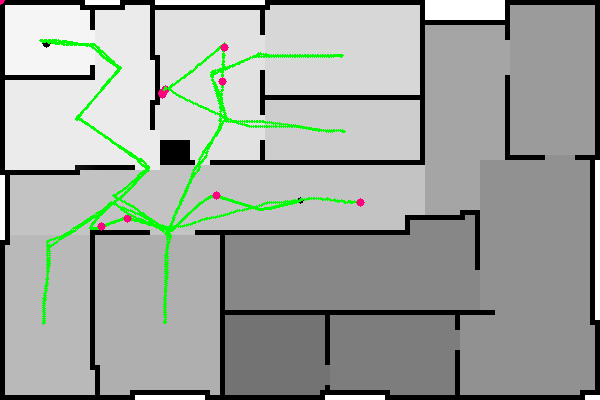
\includegraphics[width=0.85\textwidth]{../Figures/Modelbased/brushfireMarble1}
    \caption{Illustration of distance travelled for test 1, where the robots visits all 14 rooms while collecting marbles}
    \label{fig:Marble1}
  \end{subfigure}
  \hfill
  \begin{subfigure}[b]{0.49\textwidth}
    \centering
    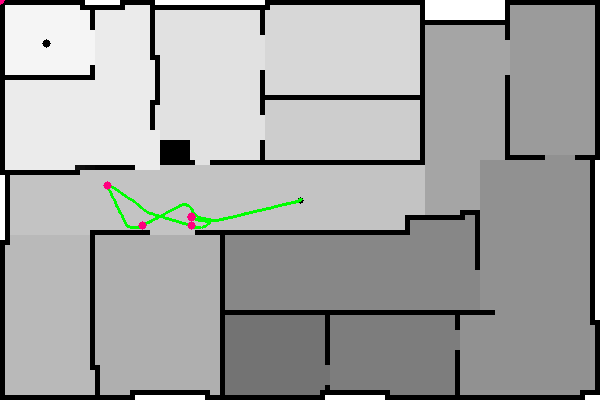
\includegraphics[width=0.85\textwidth]{../Figures/Modelbased/brushfireMarble2}
    \caption{Illustration of distance travelled for test 2, where the robots visits all 14 rooms while collecting marbles}
    \label{fig:Marble2}
  \end{subfigure}
  \caption{Illustration of distance travelled for test 1-2, where the robots visits all 14 rooms while collecting marbles}
\end{figure}
\begin{figure}[H]
  \begin{subfigure}[b]{0.49\textwidth}
    \centering
    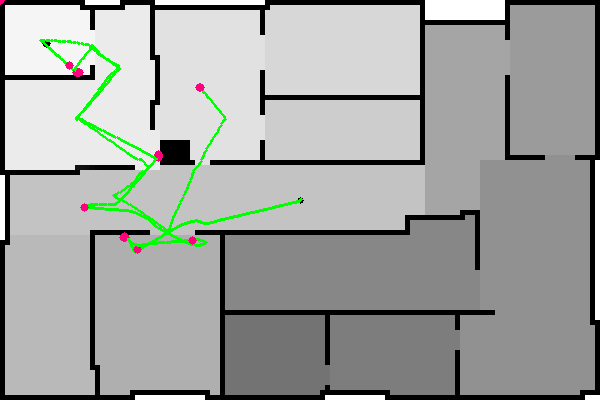
\includegraphics[width=0.85\textwidth]{../Figures/Modelbased/brushfireMarble3}
    \caption{Illustration of distance travelled for test 3, where the robots visits all 14 rooms while collecting marbles}
    \label{fig:Marble3}
  \end{subfigure}
  \hfill
  \begin{subfigure}[b]{0.49\textwidth}
    \centering
    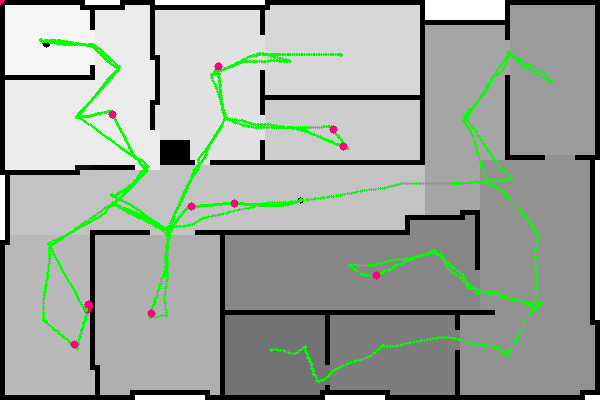
\includegraphics[width=0.85\textwidth]{../Figures/Modelbased/brushfireMarble4}
    \caption{Illustration of distance travelled for test 4, where the robots visits all 14 rooms while collecting marbles}
    \label{fig:Marble4}
  \end{subfigure}
  \hfill
  \begin{subfigure}[b]{0.49\textwidth}
  \centering
  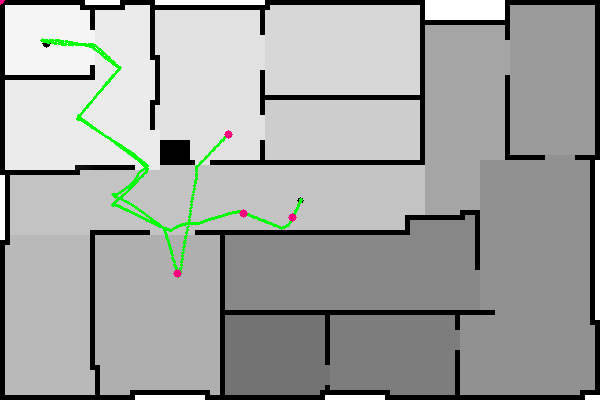
\includegraphics[width=0.85\textwidth]{../Figures/Modelbased/brushfireMarble5}
    \caption{Illustration of distance travelled for test 5, where the robots visits all 14 rooms while collecting marbles}
    \label{fig:Marble5}
  \end{subfigure}
  \hfill
  \begin{subfigure}[b]{0.49\textwidth}
    \centering
    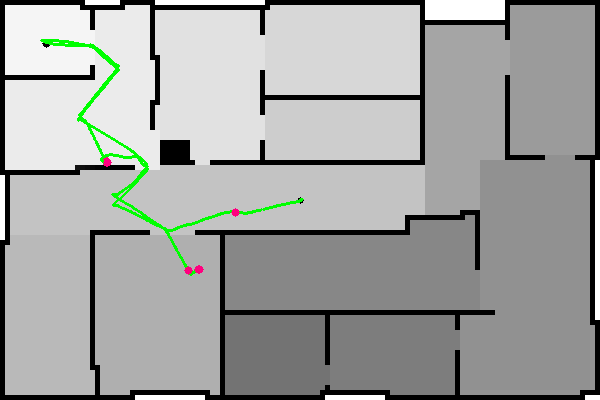
\includegraphics[width=0.85\textwidth]{../Figures/Modelbased/brushfireMarble6}
    \caption{Illustration of distance travelled for test 6, where the robots visits all 14 rooms while collecting marbles}
    \label{fig:Marble6}
  \end{subfigure}
  \hfill
  \begin{subfigure}[b]{0.49\textwidth}
  \centering
  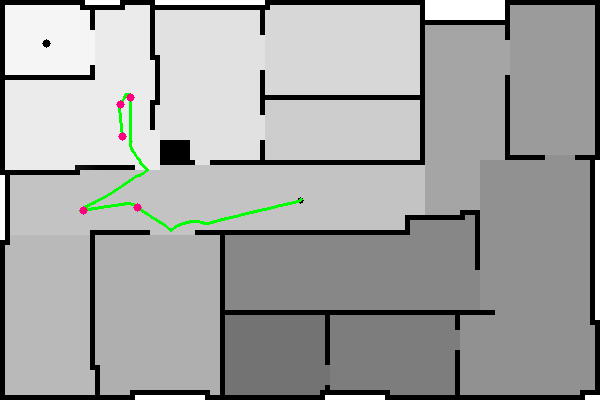
\includegraphics[width=0.85\textwidth]{../Figures/Modelbased/brushfireMarble7}
    \caption{Illustration of distance travelled for test 7, where the robots visits all 14 rooms while collecting marbles}
    \label{fig:Marble7}
  \end{subfigure}
  \hfill
  \begin{subfigure}[b]{0.49\textwidth}
    \centering
    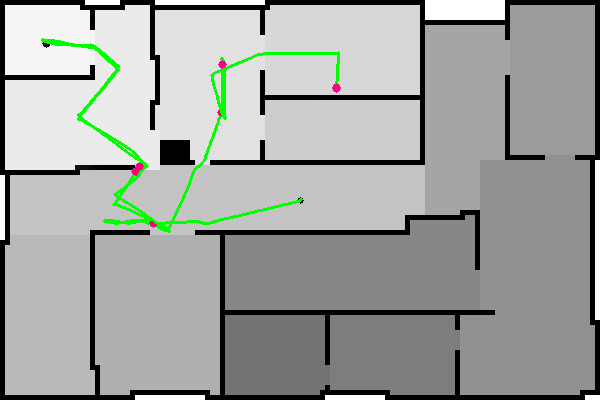
\includegraphics[width=0.85\textwidth]{../Figures/Modelbased/brushfireMarble8}
    \caption{Illustration of distance travelled for test 8, where the robots visits all 14 rooms while collecting marbles}
    \label{fig:Marble8}
  \end{subfigure}
  \hfill
  \begin{subfigure}[b]{0.49\textwidth}
  \centering
  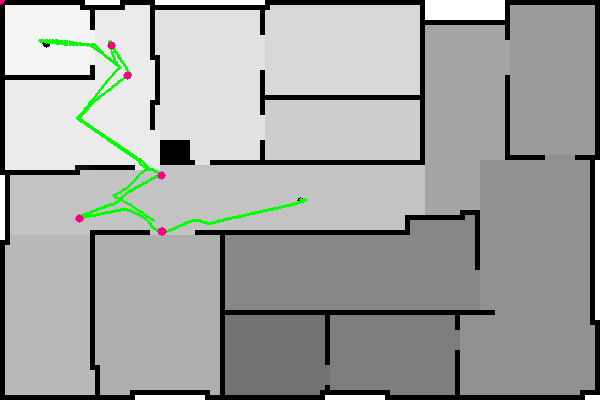
\includegraphics[width=0.85\textwidth]{../Figures/Modelbased/brushfireMarble9}
    \caption{Illustration of distance travelled for test 9, where the robots visits all 14 rooms while collecting marbles}
    \label{fig:Marble9}
  \end{subfigure}
  \hfill
  \begin{subfigure}[b]{0.49\textwidth}
    \centering
    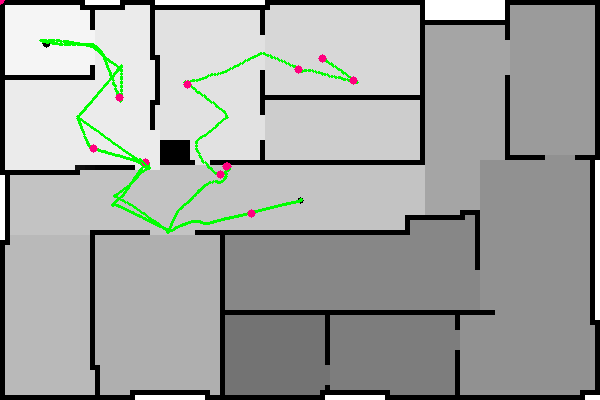
\includegraphics[width=0.85\textwidth]{../Figures/Modelbased/brushfireMarble10}
    \caption{Illustration of distance travelled for test 10, where the robots visits all 14 rooms while collecting marbles}
    \label{fig:Marble10}
  \end{subfigure}
  \caption{Illustration of distance travelled for test 3-10, where the robots visits all 14 rooms while collecting marbles}
\end{figure}
\end{document}